\subsubsection{Детекция и классификация зон притока на тестовой скважине}

\paragraph{Постановка задачи}
\par
В данной задаче рассматриваются данные тестовой скважины M. 
\par
Скважина имеет заранее предопределенные характеристики: в ней имеется четыре набора отверстий на известной глубине. Сверху находится клапан для входа газа, ниже – три группы отверстий для входа воды в группах по 144, 144 и 216 штук соответственно. Задача заключается в том, чтобы локализовать зоны этих перфораций и определить, какой флюид втекает – газ или вода. Схема скважины показана на рис.\ref{fig:hfnd_scheme}.

\begin{figure}[H]
\centering
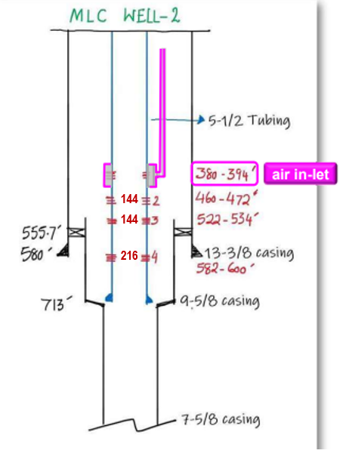
\includegraphics[width=0.5\textwidth]{PLT/hfnd_scheme.png}
\caption{Схема скважины.}
\label{fig:hfnd_scheme}
\end{figure}

\par
Для анализа используются данные прибора HFND – он содержит в себе температурный датчик и датчик пассивной акустической шумометрии. Здесь мы концентрируемся на анализе данных шумометрии. Данные записывались в диапазоне 0-100кГц с шагом 0.167м.


\paragraph{Методы и результаты}
\par
Предварительное сравнение спектрограммы со схемой перфораций показало, что отклик от притоков воды наблюдается в низких частотах, а газовый приток издает высокочастотный шум.
\par
Поэтому из всего измеряемого шумомером диапазона частот 0-100кГц для анализа мы выбрали четыре частотных диапазона:
\begin{itemize}
    \item Низкие частоты: 160-320Гц
    \item Низкие частоты, расширенные: 160-1280Гц
    \item Высокие частоты: 5-10кГц
    \item Высокие частоты, расширенные: 5-40кГц
\end{itemize}
\par
По каждому частотному диапазону в каждой точке траектории суммируются интенсивности сигналов по всем полосам, в которых производилась запись; результат показан на рис.\ref{fig:hfnd_bands}.

\begin{figure}[H]
\centering
    \subfloat[]{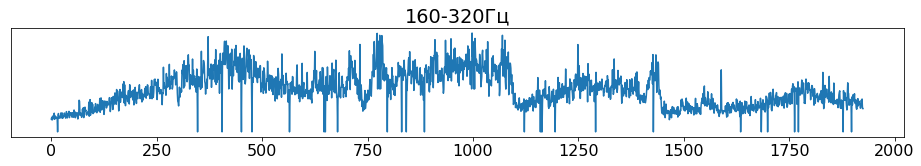
\includegraphics[width=1\textwidth]{PLT/band_1.png}}
    \vfil\vskip -20pt
    \subfloat[]{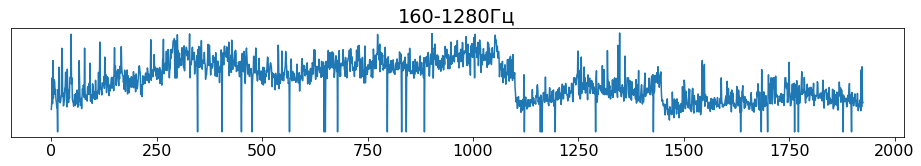
\includegraphics[width=1\textwidth]{PLT/band_2.png}}
    \vfil\vskip -20pt
    \subfloat[]{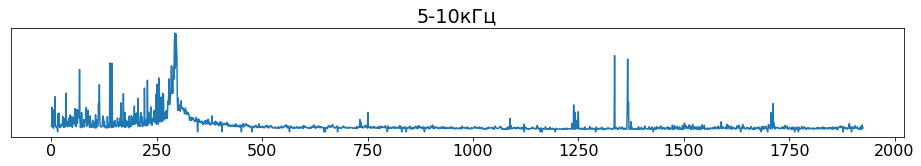
\includegraphics[width=1\textwidth]{PLT/band_3.png}}
    \vfil\vskip -20pt
    \subfloat[]{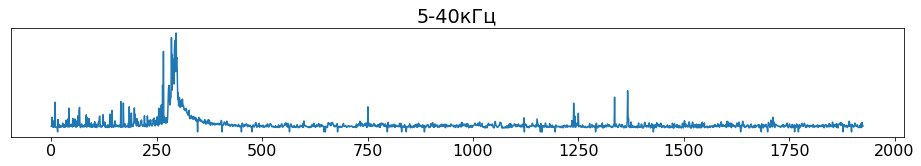
\includegraphics[width=1\textwidth]{PLT/band_4.png}}
    \vfil\vskip -20pt
\caption{Выбранные для анализа частотные диапазоны. Суммированием по всем полосам было получено усреднение интенсивности сигнала в каждой точке, которое потом используется для анализа.}
\label{fig:hfnd_bands}
\end{figure}

\par
Видно, что притоки воды можно локализовать по точкам изменения профиля интенсивности низкочастотных сигналов. Это можно объяснить следующим образом: прибор при измерении двигался снизу вверх; когда он проходил вдоль перфораций с водными притоками, притоки издавали низкочастотный шум – поэтому общая интенсивность звука увеличивалась ступенчато.
\par
Чтобы отследить это, для первых двух интервалов мы извлекаем описанные в методах разрывные кусочно-линейные профили $D_1$ и автоматически определяем участки, где скачок профиля был наибольший. Результат показан на рис.\ref{fig:hfnd_low}, скачки профиля подсвечены зеленым, искомые зоны – желтым.

\begin{figure}[H]
\centering
\subfloat[]{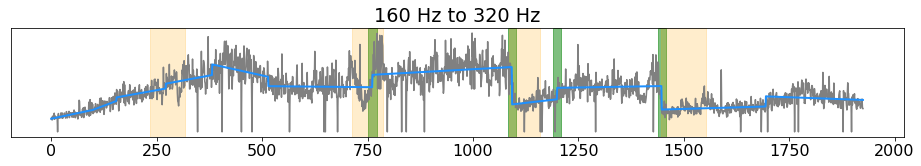
\includegraphics[width=1\textwidth]{PLT/low_1.png}}
\vfil\vskip -20pt
\subfloat[]{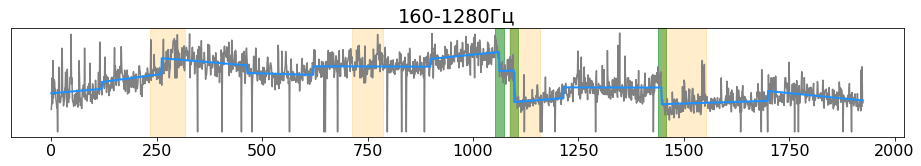
\includegraphics[width=1\textwidth]{PLT/low_2.png}}
\vfil\vskip -20pt
\caption{Результат анализа низкочастотных полос. Желтым указаны интервалы, которые хочется выделить; зеленым - полученные индикаторы. Первая полоса отвечает притоку газа, который не виден на низких частотах; другие три - водные притоки.}
\label{fig:hfnd_low}
\end{figure}

\par
Приток газа характеризуется пиком в высокочастотных диапазонах, после которого наблюдается хаотичное изменение интенсивности. Так как событие определяет пик сигнала, то мы смотрим на остаточный сигнал после выделения профиля, а не на сам профиль. 
\par
Мы хотим получить характеристику, которая служила бы индикатором хаотичности интенсивности сигнала, которая появляется после прохода зоны газового притока. Для этого сглаживаем модуль остаточного сигнала по окну и снова выделяем профиль – и ищем максимальные скачки аналогично случаю с низкими частотами. В тот момент, когда хаотичность сигнала начинает возрастать, наблюдается скачок полученной кривой. Результат показан на рис.\ref{fig:hfnd_high}.

\begin{figure}[H]
\centering
\subfloat[]{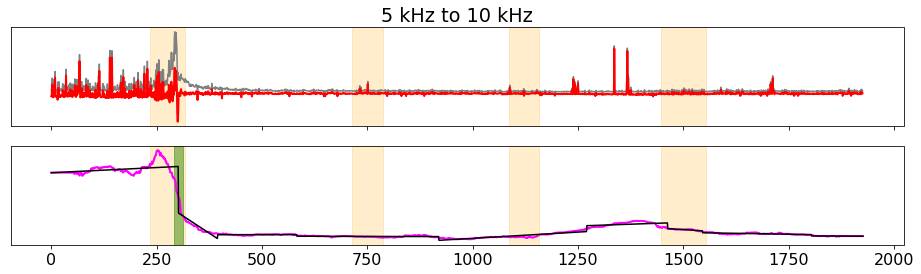
\includegraphics[width=1\textwidth]{PLT/high_1.png}}
\vfil\vskip -20pt
\subfloat[]{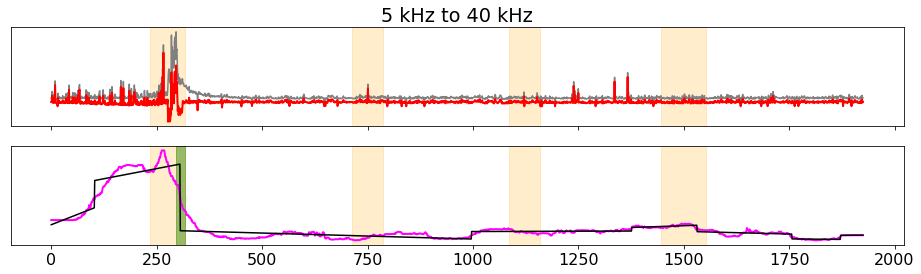
\includegraphics[width=1\textwidth]{PLT/high_2.png}}
\vfil\vskip -20pt
\caption{Результат анализа высокочастотных сигналов. Из изначального сигнала (серый) выделяется профиль и остаточный сигнал (красный). Осцилляции красного сигнала усредняются в розовый сигнал, из которого потом выделяется профиль (черный) и находится точка максимального прыжка - зеленая полоса.}
\label{fig:hfnd_high}
\end{figure}

\par
Предварительно выделенные таким образом зоны притока по низкочастотным и высокочастотным сигналам не попадают в точности в интервалы перфораций, указанные на схеме скважины. Тем не менее, их положение примерно соответствует желаемому результату; это показывает, что прибор HFND можно успешно использовать для анализа в комбинации с другими каротажными приборами.